\documentclass[12pt]{article}

%packages
%\usepackage{latexsym}
\usepackage{graphicx}
\usepackage{wrapfig}
\usepackage{color}
\usepackage{amsmath}
\usepackage{dsfont}
\usepackage{placeins}
\usepackage{amssymb}
\usepackage{skull}
\usepackage{enumerate}
\usepackage{soul}
\usepackage{alphalph}
\usepackage{hyperref}
\usepackage{enumerate}
\usepackage{listings}
%\usepackage{fancyhdr}

%\fancyhf{} % clear all header and footers
%\renewcommand{\headrulewidth}{0pt} % remove the header rule
%\fancyfoot[LE, LO]{\thepage}


%\usepackage{pstricks,pst-node,pst-tree}

%\usepackage{algpseudocode}
%\usepackage{amsthm}
%\usepackage{hyperref}
%\usepackage{mathrsfs}
%\usepackage{amsfonts}
%\usepackage{bbding}
%\usepackage{listings}
%\usepackage{appendix}
\usepackage[margin=1in]{geometry}
%\geometry{papersize={8.5in,11in},total={6.5in,9in}}
%\usepackage{cancel}
%\usepackage{algorithmic, algorithm}

\definecolor{dkgreen}{rgb}{0,0.6,0}
\definecolor{gray}{rgb}{0.5,0.5,0.5}
\definecolor{mauve}{rgb}{0.58,0,0.82}
\lstset{ %
  language=R,                     % the language of the code
  basicstyle=\footnotesize,       % the size of the fonts that are used for the code
  numbers=left,                   % where to put the line-numbers
  numberstyle=\tiny\color{gray},  % the style that is used for the line-numbers
  stepnumber=1,                   % the step between two line-numbers. If it's 1, each line
                                  % will be numbered
  numbersep=5pt,                  % how far the line-numbers are from the code
  backgroundcolor=\color{white},  % choose the background color. You must add \usepackage{color}
  showspaces=false,               % show spaces adding particular underscores
  showstringspaces=false,         % underline spaces within strings
  showtabs=false,                 % show tabs within strings adding particular underscores
  frame=single,                   % adds a frame around the code
  rulecolor=\color{black},        % if not set, the frame-color may be changed on line-breaks within not-black text (e.g. commens (green here))
  tabsize=2,                      % sets default tabsize to 2 spaces
  captionpos=b,                   % sets the caption-position to bottom
  breaklines=true,                % sets automatic line breaking
  breakatwhitespace=false,        % sets if automatic breaks should only happen at whitespace
  title=\lstname,                 % show the filename of files included with \lstinputlisting;
                                  % also try caption instead of title
  keywordstyle=\color{blue},      % keyword style
  commentstyle=\color{dkgreen},   % comment style
  stringstyle=\color{mauve},      % string literal style
  escapeinside={\%*}{*)},         % if you want to add a comment within your code
  morekeywords={*,...}            % if you want to add more keywords to the set
}

\newcommand{\qu}[1]{``#1''}
\newcommand{\spc}[1]{\\ \vspace{#1cm}}

\newcounter{probnum}
\setcounter{probnum}{1}
\newcounter{numpts}
\setcounter{numpts}{0}

%create definition to allow local margin changes
\def\changemargin#1#2{\list{}{\rightmargin#2\leftmargin#1}\item[]}
\let\endchangemargin=\endlist 

%allow equations to span multiple pages
\allowdisplaybreaks

%define colors and color typesetting conveniences
\definecolor{gray}{rgb}{0.5,0.5,0.5}
\definecolor{black}{rgb}{0,0,0}
\definecolor{white}{rgb}{1,1,1}
\definecolor{blue}{rgb}{0.5,0.5,1}
\newcommand{\inblue}[1]{\color{blue}#1 \color{black}}
\definecolor{green}{rgb}{0.133,0.545,0.133}
\newcommand{\ingreen}[1]{\color{green}#1 \color{black}}
\definecolor{yellow}{rgb}{1,0.549,0}
\newcommand{\inyellow}[1]{\color{yellow}#1 \color{black}}
\definecolor{red}{rgb}{1,0.133,0.133}
\newcommand{\inred}[1]{\color{red}#1 \color{black}}
\definecolor{purple}{rgb}{0.58,0,0.827}
\newcommand{\inpurple}[1]{\color{purple}#1 \color{black}}
\definecolor{gray}{rgb}{0.5,0.5,0.5}
\newcommand{\ingray}[1]{\color{gray}#1 \color{black}}
\definecolor{backgcode}{rgb}{0.97,0.97,0.8}
\definecolor{Brown}{cmyk}{0,0.81,1,0.60}
\definecolor{OliveGreen}{cmyk}{0.64,0,0.95,0.40}
\definecolor{CadetBlue}{cmyk}{0.62,0.57,0.23,0}

%define new math operators
\DeclareMathOperator*{\argmax}{arg\,max~}
\DeclareMathOperator*{\argmin}{arg\,min~}
\DeclareMathOperator*{\argsup}{arg\,sup~}
\DeclareMathOperator*{\arginf}{arg\,inf~}
\DeclareMathOperator*{\convolution}{\text{\Huge{$\ast$}}}
\newcommand{\infconv}[2]{\convolution^\infty_{#1 = 1} #2}
%true functions

%%%% GENERAL SHORTCUTS

\makeatletter
\newalphalph{\alphmult}[mult]{\@alph}{26}
\renewcommand{\labelenumi}{(\alphmult{\value{enumi}})}
\renewcommand{\theenumi}{\AlphAlph{\value{enumi}}}
\makeatother
%shortcuts for pure typesetting conveniences
\newcommand{\bv}[1]{\boldsymbol{#1}}

%shortcuts for compound constants
\newcommand{\BetaDistrConst}{\dfrac{\Gamma(\alpha + \beta)}{\Gamma(\alpha)\Gamma(\beta)}}
\newcommand{\NormDistrConst}{\dfrac{1}{\sqrt{2\pi\sigma^2}}}

%shortcuts for conventional symbols
\newcommand{\tsq}{\tau^2}
\newcommand{\tsqh}{\hat{\tau}^2}
\newcommand{\sigsq}{\sigma^2}
\newcommand{\sigsqsq}{\parens{\sigma^2}^2}
\newcommand{\sigsqovern}{\dfrac{\sigsq}{n}}
\newcommand{\tausq}{\tau^2}
\newcommand{\tausqalpha}{\tau^2_\alpha}
\newcommand{\tausqbeta}{\tau^2_\beta}
\newcommand{\tausqsigma}{\tau^2_\sigma}
\newcommand{\betasq}{\beta^2}
\newcommand{\sigsqvec}{\bv{\sigma}^2}
\newcommand{\sigsqhat}{\hat{\sigma}^2}
\newcommand{\sigsqhatmlebayes}{\sigsqhat_{\text{Bayes, MLE}}}
\newcommand{\sigsqhatmle}[1]{\sigsqhat_{#1, \text{MLE}}}
\newcommand{\bSigma}{\bv{\Sigma}}
\newcommand{\bSigmainv}{\bSigma^{-1}}
\newcommand{\thetavec}{\bv{\theta}}
\newcommand{\thetahat}{\hat{\theta}}
\newcommand{\thetahatmle}{\hat{\theta}_{\mathrm{MLE}}}
\newcommand{\thetavechatmle}{\hat{\thetavec}_{\mathrm{MLE}}}
\newcommand{\muhat}{\hat{\mu}}
\newcommand{\musq}{\mu^2}
\newcommand{\muvec}{\bv{\mu}}
\newcommand{\muhatmle}{\muhat_{\text{MLE}}}
\newcommand{\lambdahat}{\hat{\lambda}}
\newcommand{\lambdahatmle}{\lambdahat_{\text{MLE}}}
\newcommand{\thetahatmap}{\hat{\theta}_{\mathrm{MAP}}}
\newcommand{\thetahatmae}{\hat{\theta}_{\mathrm{MAE}}}
\newcommand{\thetahatmmse}{\hat{\theta}_{\mathrm{MMSE}}}
\newcommand{\etavec}{\bv{\eta}}
\newcommand{\alphavec}{\bv{\alpha}}
\newcommand{\minimaxdec}{\delta^*_{\mathrm{mm}}}
\newcommand{\ybar}{\bar{y}}
\newcommand{\xbar}{\bar{x}}
\newcommand{\Xbar}{\bar{X}}
\newcommand{\iid}{~{\buildrel iid \over \sim}~}
\newcommand{\inddist}{~{\buildrel ind \over \sim}~}
\newcommand{\approxdist}{~{\buildrel approx \over \sim}~}
\newcommand{\equalsindist}{~{\buildrel d \over =}~}
\newcommand{\loglik}[1]{\ell\parens{#1}}
\newcommand{\thetahatkminone}{\thetahat^{(k-1)}}
\newcommand{\thetahatkplusone}{\thetahat^{(k+1)}}
\newcommand{\thetahatk}{\thetahat^{(k)}}
\newcommand{\half}{\frac{1}{2}}
\newcommand{\third}{\frac{1}{3}}
\newcommand{\twothirds}{\frac{2}{3}}
\newcommand{\fourth}{\frac{1}{4}}
\newcommand{\fifth}{\frac{1}{5}}
\newcommand{\sixth}{\frac{1}{6}}

%shortcuts for vector and matrix notation
\newcommand{\A}{\bv{A}}
\newcommand{\At}{\A^T}
\renewcommand{\H}{\bv{H}}
\newcommand{\Ht}{\H^\top}
\newcommand{\Ainv}{\inverse{\A}}
\newcommand{\B}{\bv{B}}
\newcommand{\K}{\bv{K}}
\newcommand{\Kt}{\K^T}
\newcommand{\Kinv}{\inverse{K}}
\newcommand{\Kinvt}{(\Kinv)^T}
\newcommand{\M}{\bv{M}}
\newcommand{\Bt}{\B^T}
\newcommand{\Q}{\bv{Q}}
\newcommand{\Qt}{\Q^T}
\newcommand{\R}{\bv{R}}
\newcommand{\Rt}{\R^T}
\newcommand{\Z}{\bv{Z}}
\newcommand{\X}{\bv{X}}
\renewcommand{\b}{\bv{b}}
\newcommand{\Xsub}{\X_{\text{(sub)}}}
\newcommand{\Xsubadj}{\X_{\text{(sub,adj)}}}
\newcommand{\I}{\bv{I}}
\newcommand{\Y}{\bv{Y}}
\newcommand{\sigsqI}{\sigsq\I}
\renewcommand{\P}{\bv{P}}
\newcommand{\Psub}{\P_{\text{(sub)}}}
\newcommand{\Pt}{\P^T}
\newcommand{\Pii}{P_{ii}}
\newcommand{\Pij}{P_{ij}}
\newcommand{\IminP}{(\I-\P)}
\newcommand{\Xt}{\bv{X}^T}
\newcommand{\XtX}{\Xt\X}
\newcommand{\XtXinv}{\parens{\Xt\X}^{-1}}
\newcommand{\XtXinvXt}{\XtXinv\Xt}
\newcommand{\XXtXinvXt}{\X\XtXinvXt}
\newcommand{\x}{\bv{x}}
\newcommand{\w}{\bv{w}}
\newcommand{\onevec}{\bv{1}}
\newcommand{\oneton}{1, \ldots, n}
\newcommand{\yoneton}{y_1, \ldots, y_n}
\newcommand{\yonetonorder}{y_{(1)}, \ldots, y_{(n)}}
\newcommand{\Yoneton}{Y_1, \ldots, Y_n}
\newcommand{\iinoneton}{i \in \braces{\oneton}}
\newcommand{\onetom}{1, \ldots, m}
\newcommand{\jinonetom}{j \in \braces{\onetom}}
\newcommand{\xoneton}{x_1, \ldots, x_n}
\newcommand{\Xoneton}{X_1, \ldots, X_n}
\newcommand{\xt}{\x^T}
\newcommand{\y}{\bv{y}}
\newcommand{\yt}{\y^T}
\renewcommand{\c}{\bv{c}}
\newcommand{\ct}{\c^T}
\newcommand{\tstar}{\bv{t}^*}
\renewcommand{\u}{\bv{u}}
\renewcommand{\v}{\bv{v}}
\renewcommand{\a}{\bv{a}}
\newcommand{\s}{\bv{s}}
\newcommand{\yadj}{\y_{\text{(adj)}}}
\newcommand{\xjadj}{\x_{j\text{(adj)}}}
\newcommand{\xjadjM}{\x_{j \perp M}}
\newcommand{\yhat}{\hat{\y}}
\newcommand{\yhatsub}{\yhat_{\text{(sub)}}}
\newcommand{\yhatstar}{\yhat^*}
\newcommand{\yhatstarnew}{\yhatstar_{\text{new}}}
\newcommand{\z}{\bv{z}}
\newcommand{\zt}{\z^T}
\newcommand{\bb}{\bv{b}}
\newcommand{\bbt}{\bb^T}
\newcommand{\bbeta}{\bv{\beta}}
\newcommand{\beps}{\bv{\epsilon}}
\newcommand{\bepst}{\beps^T}
\newcommand{\e}{\bv{e}}
\newcommand{\Mofy}{\M(\y)}
\newcommand{\KofAlpha}{K(\alpha)}
\newcommand{\ellset}{\mathcal{L}}
\newcommand{\oneminalph}{1-\alpha}
\newcommand{\SSE}{\text{SSE}}
\newcommand{\SSEsub}{\text{SSE}_{\text{(sub)}}}
\newcommand{\MSE}{\text{MSE}}
\newcommand{\RMSE}{\text{RMSE}}
\newcommand{\SSR}{\text{SSR}}
\newcommand{\SST}{\text{SST}}
\newcommand{\JSest}{\delta_{\text{JS}}(\x)}
\newcommand{\Bayesest}{\delta_{\text{Bayes}}(\x)}
\newcommand{\EmpBayesest}{\delta_{\text{EmpBayes}}(\x)}
\newcommand{\BLUPest}{\delta_{\text{BLUP}}}
\newcommand{\MLEest}[1]{\hat{#1}_{\text{MLE}}}

%shortcuts for Linear Algebra stuff (i.e. vectors and matrices)
\newcommand{\twovec}[2]{\bracks{\begin{array}{c} #1 \\ #2 \end{array}}}
\newcommand{\threevec}[3]{\bracks{\begin{array}{c} #1 \\ #2 \\ #3 \end{array}}}
\newcommand{\fivevec}[5]{\bracks{\begin{array}{c} #1 \\ #2 \\ #3 \\ #4 \\ #5 \end{array}}}
\newcommand{\twobytwomat}[4]{\bracks{\begin{array}{cc} #1 & #2 \\ #3 & #4 \end{array}}}
\newcommand{\threebytwomat}[6]{\bracks{\begin{array}{cc} #1 & #2 \\ #3 & #4 \\ #5 & #6 \end{array}}}

%shortcuts for conventional compound symbols
\newcommand{\thetainthetas}{\theta \in \Theta}
\newcommand{\reals}{\mathbb{R}}
\newcommand{\complexes}{\mathbb{C}}
\newcommand{\rationals}{\mathbb{Q}}
\newcommand{\integers}{\mathbb{Z}}
\newcommand{\naturals}{\mathbb{N}}
\newcommand{\forallninN}{~~\forall n \in \naturals}
\newcommand{\forallxinN}[1]{~~\forall #1 \in \reals}
\newcommand{\matrixdims}[2]{\in \reals^{\,#1 \times #2}}
\newcommand{\inRn}[1]{\in \reals^{\,#1}}
\newcommand{\mathimplies}{\quad\Rightarrow\quad}
\newcommand{\mathlogicequiv}{\quad\Leftrightarrow\quad}
\newcommand{\eqncomment}[1]{\quad \text{(#1)}}
\newcommand{\limitn}{\lim_{n \rightarrow \infty}}
\newcommand{\limitN}{\lim_{N \rightarrow \infty}}
\newcommand{\limitd}{\lim_{d \rightarrow \infty}}
\newcommand{\limitt}{\lim_{t \rightarrow \infty}}
\newcommand{\limitsupn}{\limsup_{n \rightarrow \infty}~}
\newcommand{\limitinfn}{\liminf_{n \rightarrow \infty}~}
\newcommand{\limitk}{\lim_{k \rightarrow \infty}}
\newcommand{\limsupn}{\limsup_{n \rightarrow \infty}}
\newcommand{\limsupk}{\limsup_{k \rightarrow \infty}}
\newcommand{\floor}[1]{\left\lfloor #1 \right\rfloor}
\newcommand{\ceil}[1]{\left\lceil #1 \right\rceil}

%shortcuts for environments
\newcommand{\beqn}{\vspace{-0.25cm}\begin{eqnarray*}}
\newcommand{\eeqn}{\end{eqnarray*}}
\newcommand{\bneqn}{\vspace{-0.25cm}\begin{eqnarray}}
\newcommand{\eneqn}{\end{eqnarray}}
\newcommand{\benum}{\begin{enumerate}}
\newcommand{\eenum}{\end{enumerate}}

%shortcuts for mini environments
\newcommand{\parens}[1]{\left(#1\right)}
\newcommand{\squared}[1]{\parens{#1}^2}
\newcommand{\tothepow}[2]{\parens{#1}^{#2}}
\newcommand{\prob}[1]{\mathbb{P}\parens{#1}}
\newcommand{\littleo}[1]{o\parens{#1}}
\newcommand{\bigo}[1]{O\parens{#1}}
\newcommand{\Lp}[1]{\mathbb{L}^{#1}}
\renewcommand{\arcsin}[1]{\text{arcsin}\parens{#1}}
\newcommand{\prodonen}[2]{\bracks{\prod_{#1=1}^n #2}}
\newcommand{\mysum}[4]{\sum_{#1=#2}^{#3} #4}
\newcommand{\sumonen}[2]{\sum_{#1=1}^n #2}
\newcommand{\infsum}[2]{\sum_{#1=1}^\infty #2}
\newcommand{\infprod}[2]{\prod_{#1=1}^\infty #2}
\newcommand{\infunion}[2]{\bigcup_{#1=1}^\infty #2}
\newcommand{\infinter}[2]{\bigcap_{#1=1}^\infty #2}
\newcommand{\infintegral}[2]{\int^\infty_{-\infty} #2 ~\text{d}#1}
\newcommand{\supthetas}[1]{\sup_{\thetainthetas}\braces{#1}}
\newcommand{\bracks}[1]{\left[#1\right]}
\newcommand{\braces}[1]{\left\{#1\right\}}
\newcommand{\set}[1]{\left\{#1\right\}}
\newcommand{\abss}[1]{\left|#1\right|}
\newcommand{\norm}[1]{\left|\left|#1\right|\right|}
\newcommand{\normsq}[1]{\norm{#1}^2}
\newcommand{\inverse}[1]{\parens{#1}^{-1}}
\newcommand{\rowof}[2]{\parens{#1}_{#2\cdot}}

%shortcuts for functionals
\newcommand{\realcomp}[1]{\text{Re}\bracks{#1}}
\newcommand{\imagcomp}[1]{\text{Im}\bracks{#1}}
\newcommand{\range}[1]{\text{range}\bracks{#1}}
\newcommand{\colsp}[1]{\text{colsp}\bracks{#1}}
\newcommand{\rowsp}[1]{\text{rowsp}\bracks{#1}}
\newcommand{\tr}[1]{\text{tr}\bracks{#1}}
\newcommand{\rank}[1]{\text{rank}\bracks{#1}}
\newcommand{\proj}[2]{\text{Proj}_{#1}\bracks{#2}}
\newcommand{\projcolspX}[1]{\text{Proj}_{\colsp{\X}}\bracks{#1}}
\newcommand{\median}[1]{\text{median}\bracks{#1}}
\newcommand{\mean}[1]{\text{mean}\bracks{#1}}
\newcommand{\dime}[1]{\text{dim}\bracks{#1}}
\renewcommand{\det}[1]{\text{det}\bracks{#1}}
\newcommand{\expe}[1]{\mathbb{E}\bracks{#1}}
\newcommand{\expeabs}[1]{\expe{\abss{#1}}}
\newcommand{\expesub}[2]{\mathbb{E}_{#1}\bracks{#2}}
\newcommand{\cexpesub}[3]{\mathbb{E}_{#1}\bracks{#2~|~#3}}
\newcommand{\indic}[1]{\mathds{1}_{#1}}
\newcommand{\var}[1]{\mathbb{V}\text{ar}\bracks{#1}}
\newcommand{\sd}[1]{\mathbb{S}\text{D}\bracks{#1}}
\newcommand{\cov}[2]{\text{Cov}\bracks{#1, #2}}
\newcommand{\corr}[2]{\text{Corr}\bracks{#1, #2}}
\newcommand{\se}[1]{\text{SE}\bracks{#1}}
\newcommand{\seest}[1]{\hat{\text{SE}}\bracks{#1}}
\newcommand{\bias}[1]{\text{Bias}\bracks{#1}}
\newcommand{\partialop}[2]{\dfrac{\partial}{\partial #1}\bracks{#2}}
\newcommand{\secpartialop}[2]{\dfrac{\partial^2}{\partial #1^2}\bracks{#2}}
\newcommand{\mixpartialop}[3]{\dfrac{\partial^2}{\partial #1 \partial #2}\bracks{#3}}

%shortcuts for functions
\renewcommand{\exp}[1]{\mathrm{exp}\parens{#1}}
\renewcommand{\cos}[1]{\text{cos}\parens{#1}}
\renewcommand{\sin}[1]{\text{sin}\parens{#1}}
\newcommand{\sign}[1]{\text{sign}\parens{#1}}
\newcommand{\are}[1]{\mathrm{ARE}\parens{#1}}
\newcommand{\natlog}[1]{\ln\parens{#1}}
\newcommand{\oneover}[1]{\frac{1}{#1}}
\newcommand{\overtwo}[1]{\frac{#1}{2}}
\newcommand{\overn}[1]{\frac{#1}{n}}
\newcommand{\oneoversqrt}[1]{\oneover{\sqrt{#1}}}
\newcommand{\sqd}[1]{\parens{#1}^2}
\newcommand{\loss}[1]{\ell\parens{\theta, #1}}
\newcommand{\losstwo}[2]{\ell\parens{#1, #2}}
\newcommand{\cf}{\phi(t)}

%English language specific shortcuts
\newcommand{\ie}{\textit{i.e.} }
\newcommand{\AKA}{\textit{AKA} }
\renewcommand{\iff}{\textit{iff}}
\newcommand{\eg}{\textit{e.g.} }
\renewcommand{\st}{\textit{s.t.} }
\newcommand{\wrt}{\textit{w.r.t.} }
\newcommand{\mathst}{~~\text{\st}~~}
\newcommand{\mathand}{~~\text{and}~~}
\newcommand{\ala}{\textit{a la} }
\newcommand{\ppp}{posterior predictive p-value}
\newcommand{\dd}{dataset-to-dataset}

%shortcuts for distribution titles
\newcommand{\logistic}[2]{\mathrm{Logistic}\parens{#1,\,#2}}
\newcommand{\bernoulli}[1]{\mathrm{Bernoulli}\parens{#1}}
\newcommand{\betanot}[2]{\mathrm{Beta}\parens{#1,\,#2}}
\newcommand{\stdbetanot}{\betanot{\alpha}{\beta}}
\newcommand{\multnormnot}[3]{\mathcal{N}_{#1}\parens{#2,\,#3}}
\newcommand{\normnot}[2]{\mathcal{N}\parens{#1,\,#2}}
\newcommand{\classicnormnot}{\normnot{\mu}{\sigsq}}
\newcommand{\stdnormnot}{\normnot{0}{1}}
\newcommand{\uniform}[2]{\mathrm{U}\parens{#1,\,#2}}
\newcommand{\stduniform}{\uniform{0}{1}}
\newcommand{\exponential}[1]{\mathrm{Exp}\parens{#1}}
\newcommand{\gammadist}[2]{\mathrm{Gamma}\parens{#1, #2}}
\newcommand{\poisson}[1]{\mathrm{Poisson}\parens{#1}}
\newcommand{\binomial}[2]{\mathrm{Binomial}\parens{#1,\,#2}}
\newcommand{\rayleigh}[1]{\mathrm{Rayleigh}\parens{#1}}
\newcommand{\multinomial}[2]{\mathrm{Multinomial}\parens{#1,\,#2}}
\newcommand{\gammanot}[2]{\mathrm{Gamma}\parens{#1,\,#2}}
\newcommand{\cauchynot}[2]{\text{Cauchy}\parens{#1,\,#2}}
\newcommand{\invchisqnot}[1]{\text{Inv}\chisq{#1}}
\newcommand{\invscaledchisqnot}[2]{\text{ScaledInv}\ncchisq{#1}{#2}}
\newcommand{\invgammanot}[2]{\text{InvGamma}\parens{#1,\,#2}}
\newcommand{\chisq}[1]{\chi^2_{#1}}
\newcommand{\ncchisq}[2]{\chi^2_{#1}\parens{#2}}
\newcommand{\ncF}[3]{F_{#1,#2}\parens{#3}}

%shortcuts for PDF's of common distributions
\newcommand{\logisticpdf}[3]{\oneover{#3}\dfrac{\exp{-\dfrac{#1 - #2}{#3}}}{\parens{1+\exp{-\dfrac{#1 - #2}{#3}}}^2}}
\newcommand{\betapdf}[3]{\dfrac{\Gamma(#2 + #3)}{\Gamma(#2)\Gamma(#3)}#1^{#2-1} (1-#1)^{#3-1}}
\newcommand{\normpdf}[3]{\frac{1}{\sqrt{2\pi#3}}\exp{-\frac{1}{2#3}(#1 - #2)^2}}
\newcommand{\normpdfvarone}[2]{\dfrac{1}{\sqrt{2\pi}}e^{-\half(#1 - #2)^2}}
\newcommand{\chisqpdf}[2]{\dfrac{1}{2^{#2/2}\Gamma(#2/2)}\; {#1}^{#2/2-1} e^{-#1/2}}
\newcommand{\invchisqpdf}[2]{\dfrac{2^{-\overtwo{#1}}}{\Gamma(#2/2)}\,{#1}^{-\overtwo{#2}-1}  e^{-\oneover{2 #1}}}
\newcommand{\uniformdiscrete}[1]{\mathrm{Uniform}\parens{\braces{#1}}}
\newcommand{\exponentialpdf}[2]{#2\exp{-#2#1}}
\newcommand{\poissonpdf}[2]{\dfrac{e^{-#1} #1^{#2}}{#2!}}
\newcommand{\binomialpdf}[3]{\binom{#2}{#1}#3^{#1}(1-#3)^{#2-#1}}
\newcommand{\rayleighpdf}[2]{\dfrac{#1}{#2^2}\exp{-\dfrac{#1^2}{2 #2^2}}}
\newcommand{\gammapdf}[3]{\dfrac{#3^#2}{\Gamma\parens{#2}}#1^{#2-1}\exp{-#3 #1}}
\newcommand{\cauchypdf}[3]{\oneover{\pi} \dfrac{#3}{\parens{#1-#2}^2 + #3^2}}
\newcommand{\Gammaf}[1]{\Gamma\parens{#1}}

%shortcuts for miscellaneous typesetting conveniences
\newcommand{\notesref}[1]{\marginpar{\color{gray}\tt #1\color{black}}}

%%%% DOMAIN-SPECIFIC SHORTCUTS

%Real analysis related shortcuts
\newcommand{\zeroonecl}{\bracks{0,1}}
\newcommand{\forallepsgrzero}{\forall \epsilon > 0~~}
\newcommand{\lessthaneps}{< \epsilon}
\newcommand{\fraccomp}[1]{\text{frac}\bracks{#1}}

%Bayesian related shortcuts
\newcommand{\yrep}{y^{\text{rep}}}
\newcommand{\yrepisq}{(\yrep_i)^2}
\newcommand{\yrepvec}{\bv{y}^{\text{rep}}}


%Probability shortcuts
\newcommand{\SigField}{\mathcal{F}}
\newcommand{\ProbMap}{\mathcal{P}}
\newcommand{\probtrinity}{\parens{\Omega, \SigField, \ProbMap}}
\newcommand{\convp}{~{\buildrel p \over \rightarrow}~}
\newcommand{\convLp}[1]{~{\buildrel \Lp{#1} \over \rightarrow}~}
\newcommand{\nconvp}{~{\buildrel p \over \nrightarrow}~}
\newcommand{\convae}{~{\buildrel a.e. \over \longrightarrow}~}
\newcommand{\convau}{~{\buildrel a.u. \over \longrightarrow}~}
\newcommand{\nconvau}{~{\buildrel a.u. \over \nrightarrow}~}
\newcommand{\nconvae}{~{\buildrel a.e. \over \nrightarrow}~}
\newcommand{\convd}{~{\buildrel \mathcal{D} \over \rightarrow}~}
\newcommand{\nconvd}{~{\buildrel \mathcal{D} \over \nrightarrow}~}
\newcommand{\withprob}{~~\text{w.p.}~~}
\newcommand{\io}{~~\text{i.o.}}

\newcommand{\Acl}{\bar{A}}
\newcommand{\ENcl}{\bar{E}_N}
\newcommand{\diam}[1]{\text{diam}\parens{#1}}

\newcommand{\taua}{\tau_a}

\newcommand{\myint}[4]{\int_{#2}^{#3} #4 \,\text{d}#1}
\newcommand{\laplacet}[1]{\mathscr{L}\bracks{#1}}
\newcommand{\laplaceinvt}[1]{\mathscr{L}^{-1}\bracks{#1}}
\renewcommand{\min}[1]{\text{min}\braces{#1}}

\newcommand{\Vbar}[1]{\bar{V}\parens{#1}}
\newcommand{\expnegrtau}{\exp{-r\tau}}
\newcommand{\cprob}[2]{\prob{#1~|~#2}}

%%% problem typesetting
\newcommand{\problem}{\vspace{0.2cm} \noindent {\large{\textsf{Problem \arabic{probnum}~}}} \addtocounter{probnum}{1}}
%\newcommand{\easyproblem}{\ingreen{\noindent \textsf{Problem \arabic{probnum}~}} \addtocounter{probnum}{1}}
%\newcommand{\intermediateproblem}{\noindent \inyellow{\textsf{Problem \arabic{probnum}~}} \addtocounter{probnum}{1}}
%\newcommand{\hardproblem}{\inred{\noindent \textsf{Problem \arabic{probnum}~}} \addtocounter{probnum}{1}}
%\newcommand{\extracreditproblem}{\noindent \inpurple{\textsf{Problem \arabic{probnum}~}} \addtocounter{probnum}{1}}

\newcommand{\easysubproblem}{\ingreen{\item}}
\newcommand{\intermediatesubproblem}{\inyellow{\item}}
\newcommand{\hardsubproblem}{\inred{\item}}
\newcommand{\extracreditsubproblem}{\inpurple{\item}}
%\newcommand{\subquestionwithpoints}[1]{\addtocounter{numpts}{#1} \item \ingray{[#1 pt]}~~} %  / \arabic{numpts} pts
\newcommand{\subquestionwithpoints}[1]{\addtocounter{numpts}{#1} \item \ingray{[#1 pt / \arabic{numpts} pts]}~~}  

\newtoggle{professormode}
\toggletrue{professormode} %STUDENTS: DELETE or COMMENT this line



\title{MATH 390.4 / 650.2 Spring 2018 Homework \#5t}

\author{Professor Adam Kapelner} %STUDENTS: write your name here

\iftoggle{professormode}{
\date{Due 11:59PM Monday, May 14, 2018 under the door of KY604 \\ \vspace{0.5cm} \small (this document last updated \today ~at \currenttime)}
}

\renewcommand{\abstractname}{Instructions and Philosophy}

\begin{document}
\maketitle

\iftoggle{professormode}{
\begin{abstract}
The path to success in this class is to do many problems. Unlike other courses, exclusively doing reading(s) will not help. Coming to lecture is akin to watching workout videos; thinking about and solving problems on your own is the actual ``working out.''  Feel free to \qu{work out} with others; \textbf{I want you to work on this in groups.}

Reading is still \textit{required}. For this homework set, read about all the concepts introduced in class online e.g. probabilistic classification, the logistic link function, performance characteristics of binary classification, asymmetric cost / reward classifiers. This is your responsibility to supplement in-class with your own readings. %Also, read ch 3--6 in Silver.

The problems below are color coded: \ingreen{green} problems are considered \textit{easy} and marked \qu{[easy]}; \inorange{yellow} problems are considered \textit{intermediate} and marked \qu{[harder]}, \inred{red} problems are considered \textit{difficult} and marked \qu{[difficult]} and \inpurple{purple} problems are extra credit. The \textit{easy} problems are intended to be ``giveaways'' if you went to class. Do as much as you can of the others; I expect you to at least attempt the \textit{difficult} problems. 

This homework is worth 100 points but the point distribution will not be determined until after the due date. See syllabus for the policy on late homework.

Up to 10 points are given as a bonus if the homework is typed using \LaTeX. Links to instaling \LaTeX~and program for compiling \LaTeX~is found on the syllabus. You are encouraged to use \url{overleaf.com}. If you are handing in homework this way, read the comments in the code; there are two lines to comment out and you should replace my name with yours and write your section. The easiest way to use overleaf is to copy the raw text from hwxx.tex \emph{and} preamble.tex into two new overleaf tex files with the same name. If you are asked to make drawings, you can take a picture of your handwritten drawing and insert them as figures or leave space using the \qu{$\backslash$vspace} command and draw them in after printing or attach them stapled.

The document is available with spaces for you to write your answers. If not using \LaTeX, print this document and write in your answers. I do not accept homeworks which are \textit{not} on this printout. Keep this first page printed for your records.

\end{abstract}

\thispagestyle{empty}
\vspace{1cm}
NAME: \line(1,0){380}
\clearpage
}

\end{document}

\problem{These are questions about Silver's book, chapters ...  For all parts in this question, answer using notation from class (i.e. $t ,f, g, h^*, \delta, \epsilon, e, t, z_1, \ldots, z_t, \mathbb{D}, \mathcal{H}, \mathcal{A}, \mathcal{X}, \mathcal{Y}, X, y, n, p, x_{\cdot 1}, \ldots, x_{\cdot p}$, $x_{1 \cdot}, \ldots, x_{n \cdot}$, etc. and also we now have $f_{pr}, h^*_{pr}, g_{pr}, p_{th}$, etc from probabilistic classification as well as different types of validation schemes). }

\begin{enumerate}

\easysubproblem{What algorithm that we studied in class is PECOTA most similar to?}\spc{1}

\easysubproblem{Is baseball performance as a function of age a linear model? Discuss.}\spc{2}

\intermediatesubproblem{How can baseball scouts do better than a prediction system like PECOTA?}\spc{4}

\intermediatesubproblem{Why hasn't anyone (at the time of the writing of Silver's book) taken advantage of Pitch f/x data to predict future success?}\spc{4}

\hardsubproblem{Chapter 4 is all about predicting weather. Broadly speaking, what is the problem with weather predictions? Make sure you use the framework and notation from class. This is not an easy question and we will discuss in class. Do your best.}\spc{6}

\easysubproblem{Why does the weatherman lie about the chance of rain? And where should you go if you want honest forecasts?}\spc{2}

\hardsubproblem{Chapter 5 is all about predicting earthquakes. Broadly speaking, what is the problem with earthquake predictions? It is \textit{not} the same as the problem of predicting weather. Read page 162 a few times. Make sure you use the framework and notation from class.}\spc{6}

\easysubproblem{Silver has quite a whimsical explanation of overfitting on page 163 but it is really educational! What is the nonsense predictor in the model he describes?}\spc{2}


\easysubproblem{John von Neumann was credited with saying that \qu{with four parameters I can fit an elephant and with five I can make him wiggle his trunk}. What did he mean by that and what is the message to you, the budding data scientist? }\spc{5}

\hardsubproblem{Chapter 6 is all about predicting unemployment, an index of macroeconomic performance of a country. Broadly speaking, what is the problem with unemployment predictions? It is \textit{not} the same as the problem of predicting weather or earthquakes. Make sure you use the framework and notation from class.}\spc{6}

\extracreditsubproblem{Many times in this chapter Silver says something on the order of \qu{you need to have theories about how things function in order to make good predictions.} Do you agree? Discuss.}\spc{4}


\end{enumerate}


\problem{This question is about validation for the supervised learning problem with one fixed $\mathbb{D}$.}


\begin{enumerate}

\easysubproblem{For one fixed $\mathcal{H}$ and $\mathcal{A}$ (i.e. one model), write below the steps to do a simple validation and include the final step which is shipping the final $g$.}\spc{6}

\easysubproblem{For one fixed $\mathcal{H}$ and $\mathcal{A}$ (i.e. one model), write below the steps to do a $K$-fold cross validation and include the final step which is shipping the final $g$.}\spc{10}

\intermediatesubproblem{For one fixed $\mathcal{H}$ and $\mathcal{A}$ (i.e. one model), write below the steps to do a bootstrap validation and include the final step which is shipping the final $g$.}\spc{10}

\intermediatesubproblem{For one fixed $\mathcal{H}_1, \ldots \mathcal{H}_M$ and $\mathcal{A}$ (i.e. $M$ different models), write below the steps to do a simple validation and include the final step which is shipping the final $g$.}\spc{22}

\hardsubproblem{For one fixed $\mathcal{H}_1, \ldots \mathcal{H}_M$ and $\mathcal{A}$ (i.e. $M$ different models), write below the steps to do a $K$-fold cross validation and include the final step which is shipping the final $g$. This is not an easy problem! There are a lot of steps and a lot to keep track of...}\spc{22}


\end{enumerate}


\problem{This question is about ridge regression --- an alternative to OLS.}


\begin{enumerate}

\intermediatesubproblem{Imagine we are in the \qu{Luis situation} where we have $\X$ with dimension $n \times (p+1)$ but $p+1 > n$ and we still want to do OLS. Why would the OLS solution we found previously break down in this case?}\spc{4}

\intermediatesubproblem{We will embark now to provide a solution for this case. The solution will also give nice results for other situations besides the Luis situation as well. First, assume $\lambda$ is a positive constant and demonstrate that the expression $\lambda \normsq{\w} = \w^\top (\lambda \I) \w$ i.e. it can be expressed as a quadratic form where $\lambda\I$ is the determining matrix. We will call this term $\lambda \normsq{\w}$ the \qu{ridge penalty}.}\spc{3}


\easysubproblem{Write the $\mathcal{H}$ for OLS below where there parameter is the $\w$ vector. $\w \in$ ?}\spc{1}

\easysubproblem{Write the error objective function that OLS minimizes using vectors, then expand the terms similar to the previous homework assignment.}\spc{1}

\easysubproblem{Now add the ridge penalty $\lambda \normsq{\w}$ to the expanded form you just found and write it below. We will term this two-part error function the \qu{ridge objective}.}\spc{1}

\easysubproblem{Note that the ridge objective looks a bit like the hinge loss we spoke about when we were learning about support vector machines. There are two pieces of this error function in counterbalance. When this is minimized, describe conceptually what is going on.}\spc{5}

\intermediatesubproblem{Now, the ridge penalty term as a quadratic form can be combined with the last term in the least squares error from OLS. Do this, then use the rules of vector derivatives we learned to take $d/d\w$ and write the answer below.}\spc{2}

\easysubproblem{Now set that derivative equal to zero. What matrix needs to be invertible to solve?}\spc{2}

\hardsubproblem{There's a theorem that says \textit{positive definite} matrices are invertible. A matrix is said to be positive definite if every quadratic form is positive for all vectors i.e. if $\forall \z \neq \zerovec~~ \z^\top A \z > 0$ then $A$ is positive definite. Prove this matrix from the previous question is positive definite.}\spc{5}

\easysubproblem{Now that it's positive definite (and thus invertible), solve for the $\w$ that is the argmin of the ridge objective, call it $\b_{ridge}$. Note that this is called the \qu{ridge estimator} and computing it is called \qu{ridge regression} and it was invented by Hoerl and Kennard in 1970.}\spc{3}


\easysubproblem{Did we just figure out a way out of Luis's situation? Explain.}\spc{3}

\intermediatesubproblem{It turns out in the Luis situation, many of the values of the entries of $\b_{ridge}$ are close to 0. Why should that be? Can you explain now conceptually how ridge regression works?}\spc{3}

\easysubproblem{Find $\yhat$ as a function of $\y$ using $\b_{ridge}$. Is $\yhat$ an orthogonal projection of $\y$ onto the column space of $\X$?}\spc{3}

\extracreditsubproblem{Show that this $\yhat$ is an orthogonal projection of $\y$ onto the column space of some matrix $\X_{ridge}$ (which is not $\X$!) and explain how to construct $\X_{ridge}$ on a separate page.}\spc{0}

\easysubproblem{Is the $\mathcal{H}$ for OLS the same as the $\mathcal{H}$ for ridge regression? Yes/no. \\ Is the $\mathcal{A}$ for OLS the same as the $\mathcal{A}$ for ridge regression? Yes/no.}\spc{-0.5}

\intermediatesubproblem{What is a good way to pick the value of $\lambda$, the hyperparameter of the $\mathcal{A}$ = ridge?}\spc{1}




\easysubproblem{In classification via $\mathcal{A}$ = support vector machines with hinge loss, how should we pick the value of $\lambda$? Hint: same as previous question!}\spc{1}



\extracreditsubproblem{Besides the Luis situation, in what other situations will ridge regression save the day?}\spc{3}


\hardsubproblem{The ridge penalty is beautiful because you were able to take the derivative and get an analytical solution. Consider the following algorithm:

\beqn
\b_{lasso} = \argmin_{\w~\in~\reals^{p + 1}} \braces{(\y - \X\w)^\top(\y - \X\w) + \lambda \norm{\w}^1}
\eeqn

This penalty is called the \qu{lasso penalty} and it is different from the ridge penalty in that it is not the norm of $\w$ squared but just the norm of $\w$. It turns out this algorithm (even though it has no closed form analytic solution and must be solved numerically a la the SVM) is very useful! In \qu{lasso regression} the values of $\b_{lasso}$ are not shrunk \textit{towards} 0 they are harshly punished \textit{directly to} 0! How do you think lasso regression would be useful in data science? Feel free to look at the Internet and write a few sentences below.}~\spc{6}

\easysubproblem{Is the $\mathcal{H}$ for OLS the same as the $\mathcal{H}$ for lasso regression? Yes/no. \\ Is the $\mathcal{A}$ for OLS the same as the $\mathcal{A}$ for lasso regression? Yes/no.}\spc{-0.5}

\end{enumerate}

\problem{These are questions about non-parametric regression.}


\begin{enumerate}

\easysubproblem{In problem 1, we talked about schemes to validate algorithms which tried $M$ different prespecified models. Where did these models come from?}\spc{4}

\intermediatesubproblem{What is the weakness in using $M$ pre-specified models?}\spc{5}

\hardsubproblem{Explain the steps clearly in forward stepwise linear regression.}\spc{6}

\hardsubproblem{Explain the steps clearly in \emph{backwards} stepwise linear regression.}\spc{7}

\intermediatesubproblem{What is the weakness(es) in this stepwise procedure?}\spc{4}

\easysubproblem{Define \qu{non-parametric regression}. What problem(s) does it solve? What are its goals? Discuss.}\spc{7}

\intermediatesubproblem{Provide the steps for the regression tree (the one algorithm we discussed in class) below.}\spc{10}


\easysubproblem{Consider the following data 

\begin{figure}[htp]
\centering
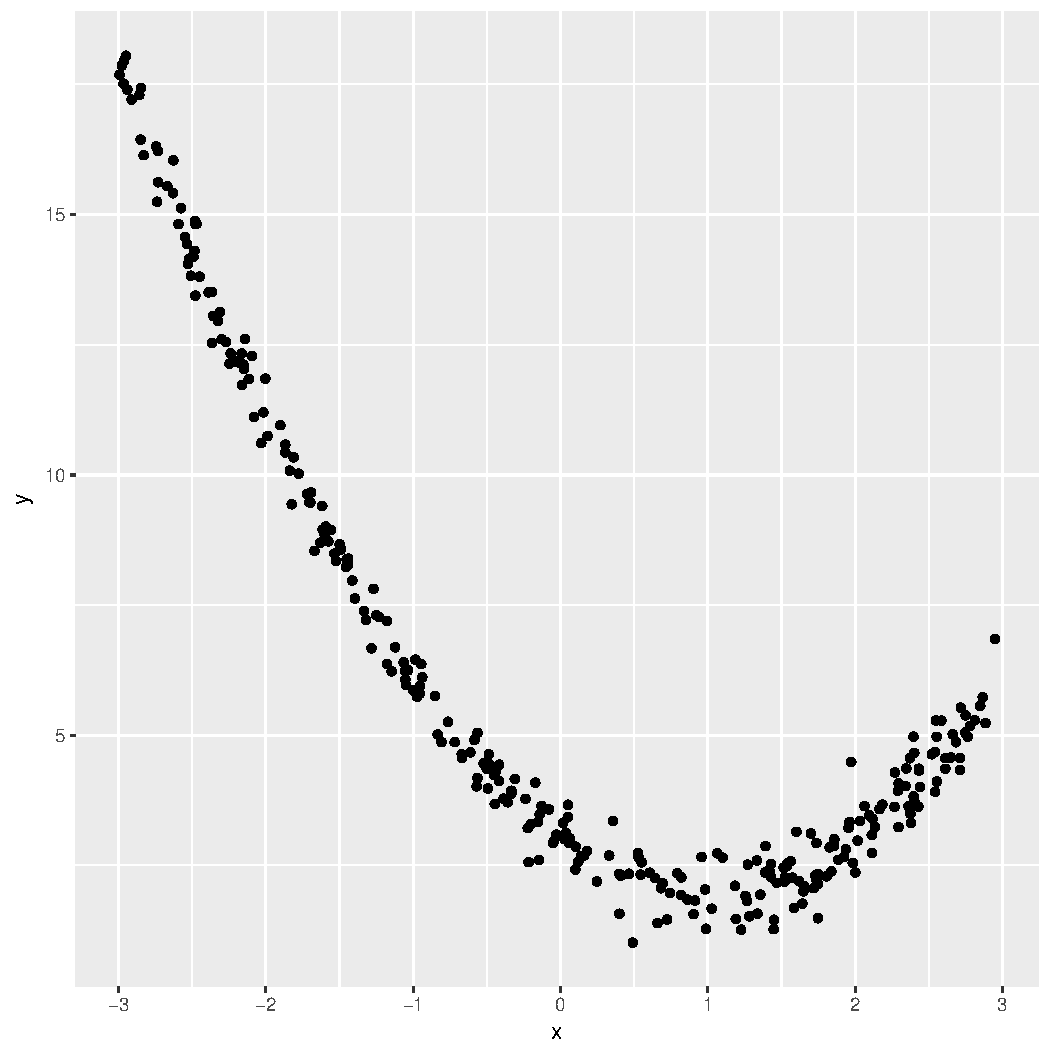
\includegraphics[width=3in]{curvy}
\end{figure}

Create a tree with maximum depth 1 (i.e one split at the root node) and plot $g$ above.}~\spc{4}


\easysubproblem{Now add a second split to the tree and plot $g$ below.

\begin{figure}[htp]
\centering
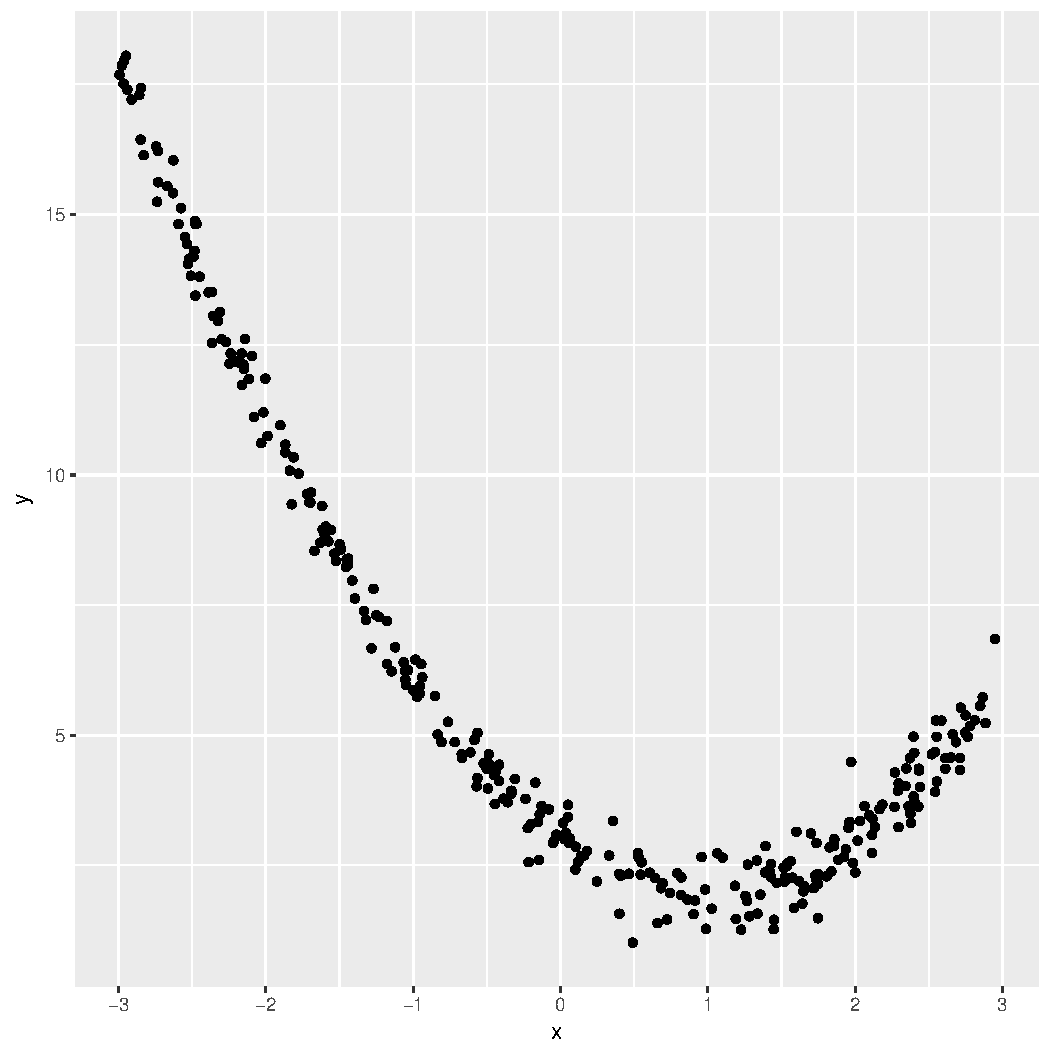
\includegraphics[width=3in]{curvy}
\end{figure}

}~\spc{-0.5}


\easysubproblem{Now add a third split to the tree and plot $g$ below.

\begin{figure}[htp]
\centering
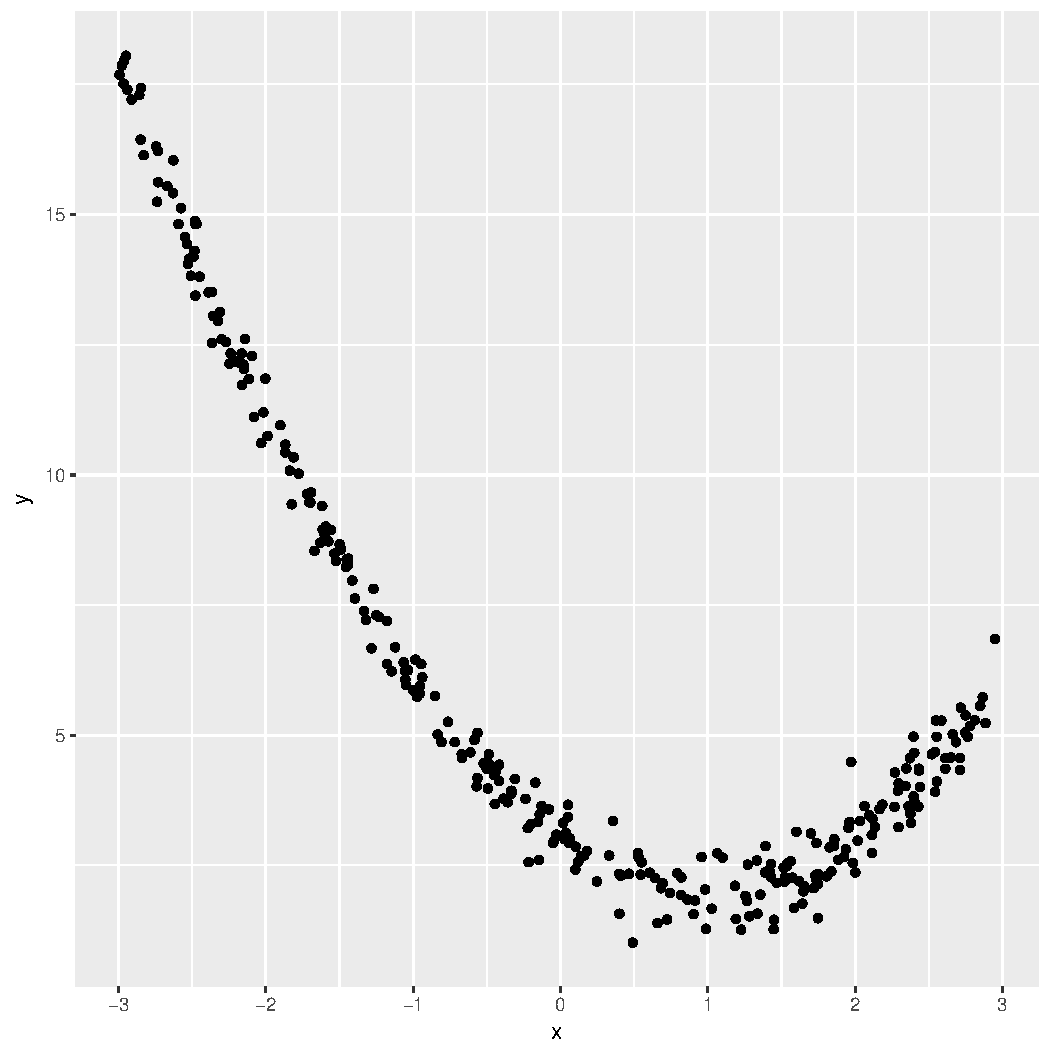
\includegraphics[width=3in]{curvy}
\end{figure}

}~\spc{5}


\easysubproblem{Now add a fourth split to the tree and plot $g$ below.

\begin{figure}[htp]
\centering
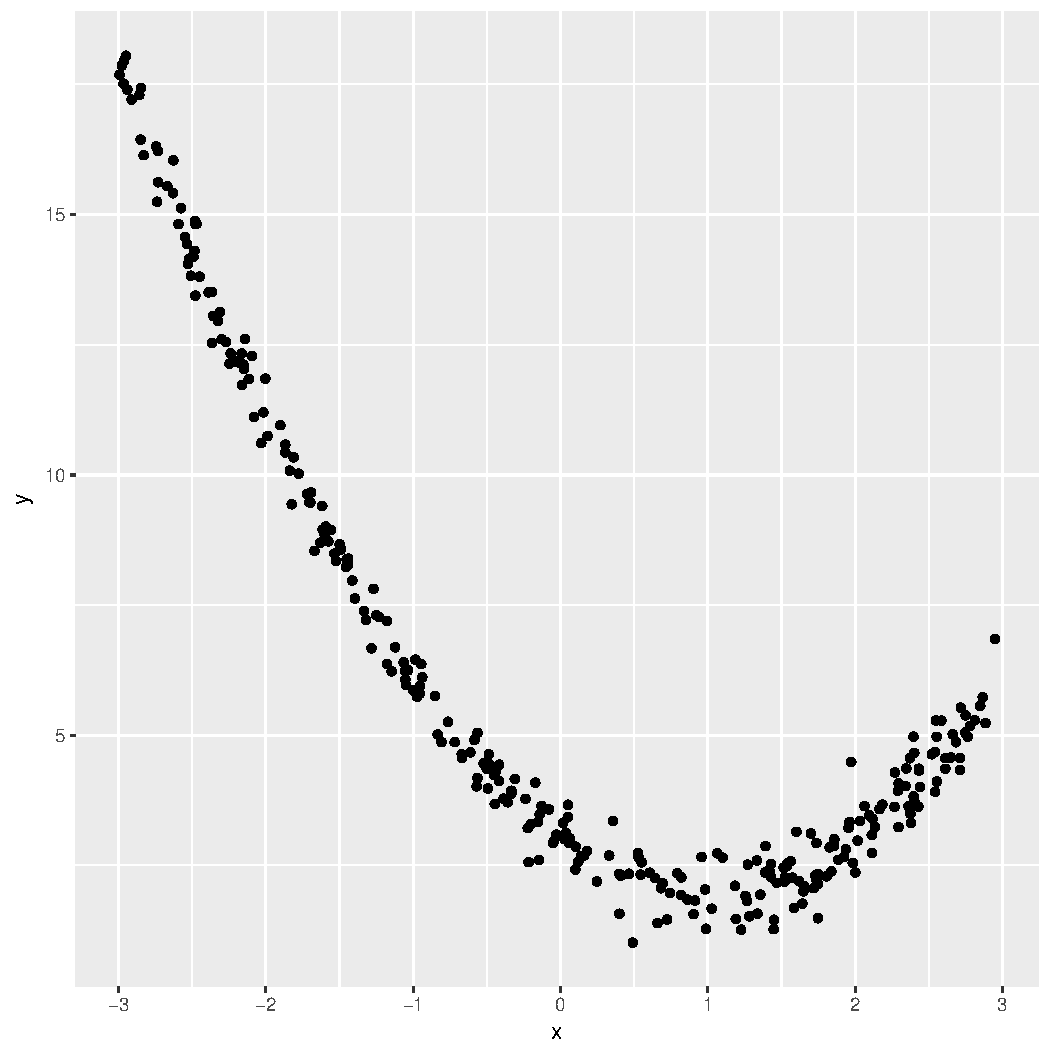
\includegraphics[width=3in]{curvy}
\end{figure}

}~\spc{-0.5}

\easysubproblem{Draw a tree diagram of $g$ below indicating which nodes are the root, inner nodes and leaves. Indicate split rules and leaf values clearly.}\spc{15}



\easysubproblem{Plot $g$ below for the mature tree with the default $N_0 =$ \texttt{nodesize} hyperparameter.

\begin{figure}[htp]
\centering
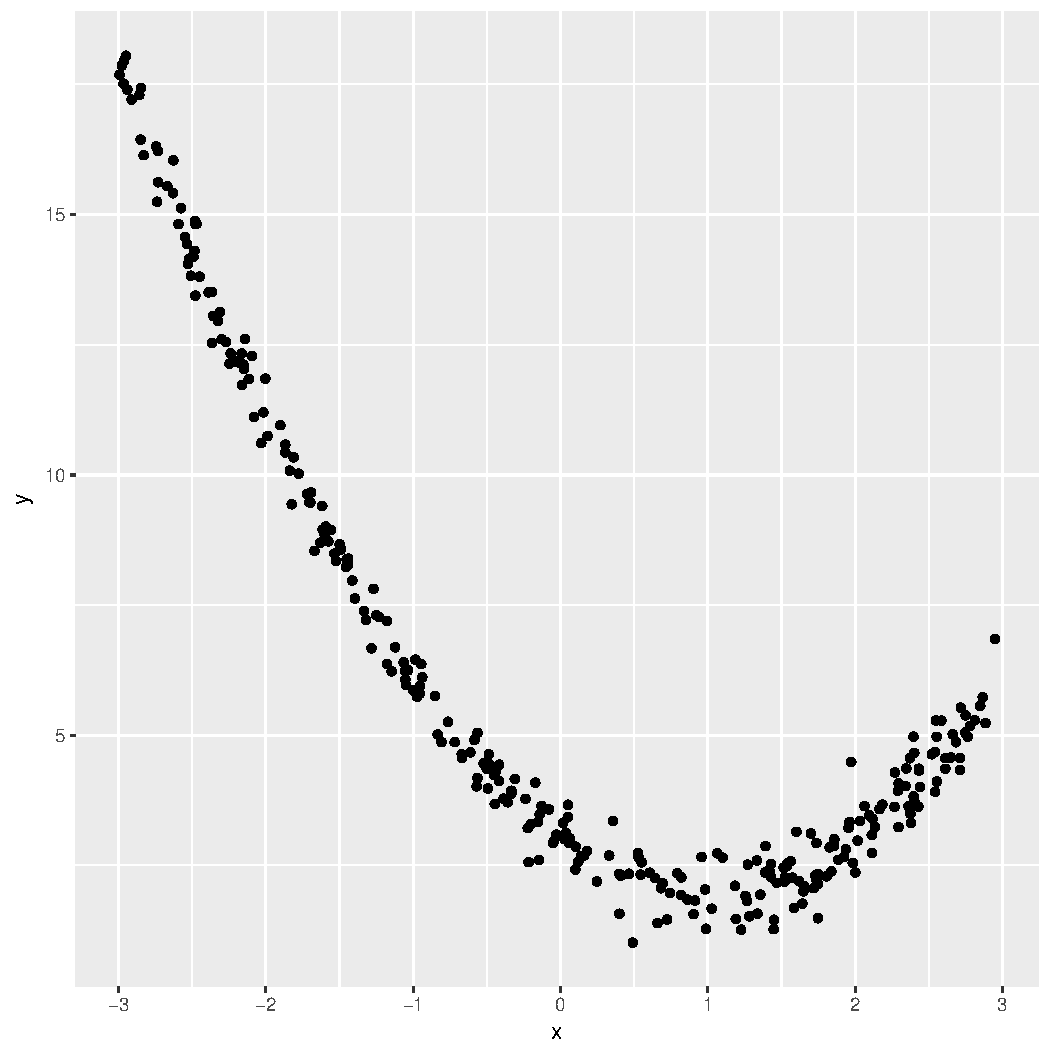
\includegraphics[width=3in]{curvy}
\end{figure}

}~\spc{-0.5}


\easysubproblem{If $N_0 =1$, what would likely go wrong?}\spc{2}

\easysubproblem{How should you pick the $N_0 =$ \texttt{nodesize} hyperparameter in practice?}\spc{2}


\end{enumerate}


\problem{These are questions about classification trees.}


\begin{enumerate}

\easysubproblem{How are classification trees different than regression trees?}\spc{2}

\intermediatesubproblem{What are the steps in the classification tree algorithm?}\spc{12}


\end{enumerate}

\problem{These are questions about measuring performance of a classifier.}

\begin{enumerate}

\easysubproblem{What is a confusion table?}\spc{8}


Consider the following in-sample confusion table where \qu{$>50$K} is the positive class:

\begin{Verbatim}
       y_hats_train
y_train <=50K >50K
  <=50K  3475  262
  >50K    471  792
\end{Verbatim}

\easysubproblem{Calculate the following: $n$ (sample size) = \\~\\
$FP$ (false positives) = \\~\\
$TP$ (true positives) = \\~\\
$FN$ (false negatives) = \\~\\
$TN$ (true negatives) = \\~\\
$\#P$ (number positive) = \\~\\
$\#N$ (number negative) = \\~\\
$\#PP$ (number predicted positive) = \\~\\
$\#PN$ (number predicted negative) = \\~\\
$\#P / n$ (prevalence / marginal rate / base rate) = \\~\\
$(FP + FN) / n$ (misclassification error) = \\~\\
$(TP + TN) / n$ (accuracy) = \\~\\
$TP / \#PP$ (precision) = \\~\\
$TP / \#P$ (recall, sensitivity, true positive rate, TPR) = \\~\\
$2 / (\text{recall}^{-1} + \text{precision}^{-1})$ (F1 score) = \\~\\
$FP / \#PP$ (false discovery rate, FDR) = \\~\\
$FP / \#N$ (false positive rate, FPR) = \\~\\ %false alarm rate 
$FN / \#PN$ (false omission rate, FOR) = \\~\\
$FN / \#P$ (false negative rate, FNR) = %miss rate 
}

\easysubproblem{Why is FPR also called the \qu{false alarm rate}?}\spc{4}

\easysubproblem{Why is FNR also called the \qu{miss rate}?}\spc{4}


\easysubproblem{Below let the red icons be the positive class and the blue icons be the negative class. 


\begin{figure}[htp]
\centering
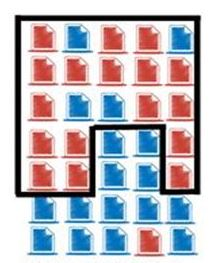
\includegraphics[width=1.5in]{precision_recall.jpg}
\end{figure}

The icons included inside the black border are those that have $\hat{y} = 1$. Compute both precision and recall.}\spc{4}

\intermediatesubproblem{There is always a tradeoff of FP vs FN. However, in some situations, you will look at FPR vs. FNR. Describe such a classification scenario. It does not have to be this income amount classification problem, it can be any problem you can think of.}\spc{3}

\intermediatesubproblem{There is always a tradeoff of FP vs FN. However, in some situations, you will look at FDR vs. FOR. Describe such a classification scenario. It does not have to be this income amount classification problem, it can be any problem you can think of.}\spc{3}

\intermediatesubproblem{There is always a tradeoff of FP vs FN. However, in some situations, you will look at precision vs. recall. Describe such a classification scenario. It does not have to be this income amount classification problem, it can be any problem you can think of.}\spc{3}


\intermediatesubproblem{There is always a tradeoff of FP vs FN. However, in some situations, you will look only at an overall metric such as accuracy (or $F1$). Describe such a classification scenario. It does not have to be this income amount classification problem, it can be any problem you can think of.}\spc{4}

\end{enumerate}







\end{document}

\problem{These are questions about Silver's book, chapter 2.}


\begin{enumerate}

\intermediatesubproblem{If one's goal is to fit a model for a phenomenon $y$, what is the difference between the approaches of the hedgehog and the fox? Answer using notation from class (i.e. $t ,f, g, h^*, \delta, \epsilon, e, t, z_1, \ldots, z_t, \mathbb{D}, \mathcal{H}, \mathcal{A}, \mathcal{X}, \mathcal{Y}, X, y, n, p, x_{\cdot 1}, \ldots, x_{\cdot p}, x_{1 \cdot}, \ldots, x_{n \cdot}$, etc.). Connecting this to the modeling framework should really make you think about what Tetlock's observation means for political and historical phenomena.}\spc{4}

\easysubproblem{Why did Harry Truman like hedgehogs? Are there a lot of people that think this way?}\spc{4}


\hardsubproblem{Why is it that the more education one acquires, the less accurate one's predictions become?}\spc{4}


\easysubproblem{Why are probabilistic classifiers (i.e. algorithms that output functions that return probabilities) better than vanilla classifiers (i.e. algorithms that only return the class label)? We will move in this direction in class soon.}\spc{4}

\end{enumerate}

\problem{These are questions about Finlay's book, chapter 2-4. We will hold off on chapter 1 until we cover probability estimation after midterm 2.}


\begin{enumerate}

\easysubproblem{What term did we use in class for \qu{behavioral (outome) data}?}\spc{0}

\easysubproblem{Write about some reasons why data scientists implement models that are subpar in predictive performance (p27).}\spc{3}


\easysubproblem{In the first wine example, what is the outcome metric and what kind of supervised learning was employed?}\spc{0}

\easysubproblem{In the second wine example, what is the outcome metric and kind of supervised learning was employed?}\spc{0}


\easysubproblem{In the third chapter, why is it that some organizations cannot use predictive modeling to improve their business?}\spc{3}

\easysubproblem{In the bankruptcy case, what is the problem with merely using $g$ to obtain a $\hat{y}$ without any other information from the model?}\spc{3}

\easysubproblem{Chapter 3 talks about using the model with human judgment. Under what circumstances is this beneficial? Answer using notation from class (i.e. $t ,f, g, h^*, \delta, \epsilon, e, t$, $z_1, \ldots, z_t, \mathbb{D}, \mathcal{H}, \mathcal{A}, \mathcal{X}, \mathcal{Y}, X, y, n, p, x_{\cdot 1}, \ldots, x_{\cdot p}, x_{1 \cdot}, \ldots, x_{n \cdot}$, etc.).}\spc{3}


\hardsubproblem{In Chapter 4 Finaly makes an interesting observation based on his experience in data science. He says most predictive models have $p \leq 30$. Why do you think this is? Discuss.}\spc{5}


\easysubproblem{He says there is \qu{almost always other data that could be acquired ... [which] doesn't always come for free}. The \qu{data} he is talking about here specifically means \qu{more predictors} i.e. increasing $p$. In what cases would someone be willing to pay for this data?}\spc{3}


\easysubproblem{Table 4 lists \qu{data types} about what type of observations?}\spc{1}

\easysubproblem{What type of data does he find in his experience to be the most important to predictive modeling? Why do you think this is so?}\spc{3}

\easysubproblem{If $x_{\cdot 17}$ was age and $x_{\cdot 18}$ is age of spouse, what is the most likely reason why adding $x_{\cdot 18}$ to $\mathbb{D}$ not be friutful for predictive ability?}\spc{3}

\hardsubproblem{What is the lifespan of a predictive model? Why does it not last forever? Answer using notation from class (i.e. $t ,f, g, h^*, \delta, \epsilon, e, t$, $z_1, \ldots, z_t, \mathbb{D}, \mathcal{H}, \mathcal{A}, \mathcal{X}, \mathcal{Y}, X, y, n, p$, $x_{\cdot 1}, \ldots, x_{\cdot p}, x_{1 \cdot}, \ldots, x_{n \cdot}$, etc.).}\spc{3}


\hardsubproblem{What does \qu{large enough to representative of the full population} (p80) mean? Answer using notation from class (i.e. $t ,f, g, h^*, \delta, \epsilon, e, t$, $z_1, \ldots, z_t, \mathbb{D}, \mathcal{H}, \mathcal{A}, \mathcal{X}, \mathcal{Y}, X, y, n, p$, $x_{\cdot 1}, \ldots, x_{\cdot p}, x_{1 \cdot}, \ldots, x_{n \cdot}$, etc.).}\spc{3}

\easysubproblem{Is there a hype about \qu{big data} i.e. including millions of observations instead of a few thousand? Discuss Finlay's opinion.}\spc{3}


\easysubproblem{What is Finlay's solution to \qu{overfitting} (p84)?}\spc{5}
\end{enumerate}


\problem{These are questions about association and correlation.}


\begin{enumerate}

\easysubproblem{Give an example of two variables that are both correlated and associated by drawing a plot.}\spc{4}

\easysubproblem{Give an example of two variables that are not correlated but are associated by drawing a plot.}\spc{4}

\easysubproblem{Give an example of two variables that are not correlated nor associated by drawing a plot.}\spc{4}

\easysubproblem{Can two variables be correlated but not associated? Explain.}\spc{4}


\end{enumerate}

\problem{These are questions about multivariate linear model fitting using the least squares algorithm.}

\begin{enumerate}

\hardsubproblem{Derive $\partialop{\c}{\c^\top A \c}$ where $\c \in \reals^n$ and $A \in \reals^{n \times n}$ but \textit{not} symmetric. Get as far as you can.}\spc{8}

\easysubproblem{Given matrix $X \in \reals^{n \times (p+1)}$, full rank and first column consisting of the $\onevec_n$ vector, rederive the least squares solution $\b$ (the vector of coefficients in the linear model shipped in the prediction function $g$). No need to rederive the facts about vector derivatives.}\spc{10}

\intermediatesubproblem{Consider the case where $p = 1$. Show that the solution for $\b$ you just derived is the same solution that we proved for simple regression in Lecture 8. That is, the first element of $\b$ is the same as $b_0 = \ybar - r \frac{s_y}{s_x}\xbar$ and the second element of $\b$ is $b_1 = r \frac{s_y}{s_x}$.} \spc{10}

\easysubproblem{If $X$ is rank deficient, how can you solve for $\b$? Explain in English.} \spc{2}

\hardsubproblem{Prove $\rank{X} =\rank{X^\top X}$.}\spc{6}

\hardsubproblem{Given matrix $X \in \reals^{n \times (p+1)}$, full rank and first column consisting of the $\onevec_n$ vector, now consider cost multiples (\qu{weights}) $c_1, c_2, \ldots, c_n$ for each mistake $e_i$. As an example, previously the mistake for the 17th observation was $e_{17} := y_{17} - \hat{y}_{17}$ but now it would be $e_{17} := c_{17} (y_{17} - \hat{y}_{17})$.  Derive the weighted least squares solution $\b$. No need to rederive the facts about vector derivatives. Hints: (1) show that SSE is a quadratic form with the matrix $C$ in the middle (2) Split this matrix up into two pieces i.e. $C = C^{\half} C^{\half}$, distribute and then foil (3) note that a scalar value equals its own transpose and (4) use the vector derivative formulas.}\spc{20}


\hardsubproblem{If $p=1$, prove $r^2 = R^2$ i.e. the linear correlation is the same as proportion of sample variance explained in a least squares linear model.}\spc{6}


\intermediatesubproblem{Prove that the point $<1,\xbar_1, \xbar_2, \ldots, \xbar_p, \bar{y}>$ is a point on the least squares linear solution.}\spc{13}

\end{enumerate}

\problem{These are questions related to the concept of orthogonal projection, QR decomposition and its relationship with least squares linear modeling.}

\begin{enumerate}

\easysubproblem{Consider least squares linear regression using a design matrix $X$ with rank $p + 1$. What are the degrees of freedom in the resulting model? What does this mean?}\spc{3}


\intermediatesubproblem{If you are orthogonally projecting the vector $\y$ onto the column space of $X$ which is of rank $p + 1$, derive the formula for $\proj{\colsp{X}}{\y}$. Is this the same as the least squares solution?}\spc{6}

\hardsubproblem{We saw that the perceptron is an \textit{iterative algorithm}. This means that it goes through multiple iterations in order to converge to a closer and closer $\w$. Why not do the same with linear least squares regression? Consider the following. Regress $\y$ using $\X$ to get $\yhat$. This generates residuals $\e$ (the leftover piece of $\y$ that wasn't explained by the regression's fit, $\yhat$). Now try again! Regress $\e$ using $\X$ and then get new residuals $\e_{new}$. Would $\e_{new}$ be closer to $\zerovec_n$ than the first $\e$? That is, wouldn't this yield a better model on iteration \#2? Yes/no and explain.}\spc{10}


\intermediatesubproblem{Prove that $Q^\top = Q^{-1}$ where $Q$ is an orthonormal matrix such that $\colsp{Q} = \colsp{X}$ and $Q$ and $X$ are both matrices $\in \reals^{n \times (p+1)}$. Hint: this is purely a linear algebra exercise.}\spc{10}


\intermediatesubproblem{Prove that the least squares projection $H = \XXtXinvXt$ is the same as $QQ^\top$.}\spc{10}

\intermediatesubproblem{Prove that an orthogonal projection onto the $\colsp{Q}$ is the same as the sum of the projections onto each column of $Q$.}\spc{10}


\hardsubproblem{Trouble in paradise. Prove that the SSE of a multivariate linear least squares model always decreases (equivalently, $R^2$ always increases) upon the addition of a new independent predictor. Keep in mind this holds true even if this new predictor has no information about the true causal inputs to the phenomenon $y$.}\spc{12}

\intermediatesubproblem{Why is this a bad thing? Explain in English.}\spc{3}



\extracreditsubproblem{Prove that $\rank{H} =\tr{H}$.}\spc{-0.5}

\end{enumerate}


\end{document}
